\documentclass[10pt,serif,mathserif,compress,hyperref={colorlinks}]{beamer}
\mode<presentation>
\usepackage{pgf}
\usepackage{pgfpages}
\usepackage[T1]{fontenc}
\usepackage[utf8]{inputenc}

\usepackage{comment}
\usepackage{geometry}
\usepackage[most]{tcolorbox}
\tcbuselibrary{skins}
\usepackage{beamerthemesplit}
\usepackage{amsmath, amsfonts, epsfig, xspace}
\usepackage{pstricks,pst-node}
\usepackage{multimedia}
\usepackage{wasysym}
\usepackage{animate}

\usepackage{graphicx}% for including figures
\usepackage{tikz}
\usetikzlibrary{positioning,decorations.pathreplacing,arrows}

\setlength{\parindent}{0pt}

%%%%%%%%%%%%%%%%%%  Couleurs %%%%%%%%%%%%%%%%%%%%%%%%%%%
\definecolor{mauve}{rgb}{0.5,0,0.7}
\definecolor{carmin}{rgb}{0.7,0,0}
\definecolor{bleu}{rgb}{0,0,0.7}
\definecolor{marron}{rgb}{0.6,0.35,0}
\definecolor{vert}{rgb}{0,0.5,0}
\definecolor{gris}{rgb}{0.9,0.9,0.9}
\definecolor{no}{rgb}{1,0.9,1}
%%%%%%%%%%%%%%%%%%%%%%%%%%%%%%%%%%%%%%%%%%%%%%%%%%%%%%%%%%

\definecolor{White}        {rgb}{1.0,1.0,1.0}

\definecolor{VeryDarkBlue} {RGB}{0,0,153}
\definecolor{DarkBlue}     {rgb}{0.0,0.0,0.6}
\definecolor{Blue}         {rgb}{0.0,0.0,1.0}
\definecolor{MidBlue}      {rgb}{0.6,0.6,1.0}
\definecolor{LightBlue}    {rgb}{0.8,0.8,1.0}
\definecolor{VeryLightBlue}{rgb}{0.9,0.9,1.0}

\definecolor{Gray}{rgb}{0.7,0.7,0.7}
\definecolor{LightGray}{rgb}{0.94,0.94,0.94}

\definecolor{DarkGreen}{rgb}{0,0.6,0}
\definecolor{MidGreen}{rgb}{0.6,1,0.6}
\definecolor{LightGreen}{rgb}{0.88,1,0.88}
\definecolor{VeryLightGreen}{rgb}{0.9,1,0.9}

\definecolor{Yellow}{rgb}{1,1,0.4}
\definecolor{MidYellow}{rgb}{1,1,0.5}
\definecolor{LightYellow}{rgb}{1,1,0.6}
\definecolor{VeryLightYellow}{rgb}{1,1,0.9}

\definecolor{DarkRed}{rgb}{0.7,0.,0.}
\definecolor{Red}{rgb}{0.8,0.,0.}
\definecolor{LightRed}{rgb}{1,0.8,0.8}
\definecolor{VeryLightRed}{rgb}{1,0.9,0.9}

\definecolor{Mauve}{rgb}{0.7,0.,0.7}

\definecolor{Magenta}{rgb}{1,0.,1}
\definecolor{LightMagenta}{rgb}{1,0.5,1}

\definecolor{Chocolate}{rgb}{0.54,0.2,.004}
\definecolor{DarkChocolate}{RGB}{103,38,.00}

\definecolor{DarkOrange}{rgb}{0.65,0.35,0.}
\definecolor{Orange}{rgb}{.9,0.4,0.}
\definecolor{LightOrange}{rgb}{1,0.8,0.5}

\definecolor{Brown}{rgb}{0.4,0.4,0.}

\definecolor{LightCyan}{rgb}{0.5,1.,1.}

\definecolor{PBG} {rgb}{1.0,1.0,0.6}
\definecolor{PTXT}{rgb}{0.2,0.2,0.0}
\definecolor{IBG} {rgb}{0.8,0.8,1.0}
\definecolor{ITXT}{rgb}{0.2,0.2,0.0}
\definecolor{OBG} {rgb}{0.8,1.0,0.8}
\definecolor{OTXT}{rgb}{0.0,0.4,0.0}

\newcommand{\CommentVeryLightBlue}[1]{{\textcolor{VeryLightBlue}{#1}}}
\newcommand{\CommentWhite}[1]{{\textcolor{White}{#1}}}

\newcommand{\VeryDarkBlue}[1]{\textcolor{DarkBlue}{#1}}
\newcommand{\DarkBlue}[1]{\textcolor{DarkBlue}{#1}}
\newcommand{\Blue}[1]{\textcolor{Blue}{#1}}
\newcommand{\LightBlue}[1]{\textcolor{LightBlue}{#1}}
\newcommand{\VeryLightBlue}[1]{\textcolor{VeryLightBlue}{#1}}

\newcommand{\DarkGreen}[1]{\textcolor{DarkGreen}{#1}}
\newcommand{\LightGreen}[1]{\textcolor{LightGreen}{#1}}
\newcommand{\VeryLightGreen}[1]{\textcolor{VeryLightGreen}{#1}}
\newcommand{\MidGreen}[1]{\textcolor{MidGreen}{#1}}

\newcommand{\DarkRed}[1]{\textcolor{DarkRed}{#1}}
\newcommand{\Red}[1]{\textcolor{red}{#1}}
\newcommand{\LightRed}[1]{\textcolor{LightRed}{#1}}
\newcommand{\VeryLightRed}[1]{\textcolor{VeryLightRed}{#1}}

\newcommand{\Gray}[1]{\textcolor{gray}{#1}}

\newcommand{\Black}[1]{\textcolor{black}{#1}}

\newcommand{\White}[1]{\textcolor{white}{#1}}

\newcommand{\Mauve}[1]{\textcolor{Mauve}{#1}}

\newcommand{\LightMagenta}[1]{\textcolor{LightMagenta}{#1}}
\newcommand{\Magenta}[1]{\textcolor{Magenta}{#1}}

\newcommand{\DarkOrange}[1]{\textcolor{DarkOrange}{#1}}
\newcommand{\Orange}[1]{\textcolor{Orange}{#1}}
\newcommand{\LightOrange}[1]{\textcolor{LightOrange}{#1}}

\newcommand{\DeepPurple}[1]{{\textcolor[rgb]{0.3,0.,0.6}{#1}}}

\newcommand{\Brown}[1]{{\textcolor{Brown}{#1}}}
\newcommand{\Chocolate}[1]{\textcolor{Chocolate}{#1}}
\newcommand{\DarkChocolate}[1]{\textcolor{DarkChocolate}{#1}}

\definecolor{DBluePy}{RGB}{ 28, 78, 99}
\definecolor{BluePy} {RGB}{ 60,110,131}
\definecolor{MBluePy}{RGB}{200,210,240}
\definecolor{LBluePy}{RGB}{220,230,240}
\definecolor{DOranPy}{RGB}{248,194,  3}
\definecolor{OranPy} {RGB}{255,220, 70}
\definecolor{GreenPy}{RGB}{237,255,204}

\newcommand{\bsh}{\textbackslash}
\newcommand{\bshbsh}{\textbackslash\textbackslash}
\newcommand{\chevrons}{\ttfamily>\hspace*{-0.25mm}>\hspace*{-0.25mm}>\hspace*{0.28mm}\xspace}
\newcommand{\M}[1]{\Mauve{#1}}
\newcommand{\DG}[1]{\DarkGreen{#1}}
\newcommand{\DR}[1]{\DarkRed{#1}}
\newcommand{\B}[1]{\Blue{#1}}
\newcommand{\BPy}[1]{\BluePy{#1}}
\newcommand{\VDB}[1]{\VeryDarkBlue{#1}}
\newcommand{\DO}[1]{\DarkOrange{#1}}
\newcommand{\Or}[1]{\Orange{#1}}
\newcommand{\Choco}[1]{\Chocolate{#1}}
\newcommand*{\truc}{\Gray{\textbullet}}

\newcommand{\bif}[1]{{\ttfamily \M{#1}}}	% Python built in function
\newcommand{\typ}[1]{{\ttfamily \M{#1}}}  % Python built in type
\newcommand{\key}[1]{{\ttfamily \Or{#1}}}
\newcommand{\str}[1]{{\ttfamily \DG{#1}}}
\newcommand{\com}[1]{{\ttfamily \DR{#1}}}
\newcommand{\out}[1]{{\ttfamily \B{#1}}}
\newcommand{\command}[1]{{\ttfamily \Choco{#1}}}
\newcommand{\code}[1]{{\ttfamily \Choco{#1}}}
\newcommand{\file}[1]{{\ttfamily \VDB{#1}}}

\newcommand{\bifBF}[1]{\textbf{\bif{#1}}}	% Python built in function
\newcommand{\typBF}[1]{\textbf{\typ{#1}}}  % Python built in type
\newcommand{\keyBF}[1]{\textbf{\key{#1}}}
\newcommand{\strBF}[1]{\textbf{\str{#1}}}
\newcommand{\comBF}[1]{\textbf{\com{#1}}}
\newcommand{\outBF}[1]{\textbf{\out{#1}}}
\newcommand{\commandBF}[1]{\textbf{\command{#1}}}
\newcommand{\codeBF}[1]{\textbf{\code{#1}}}
\newcommand{\fileBF}[1]{\textbf{\file{#1}}}

\newcommand{\bfchoco}[1]{\textbf{\Chocolate{#1}}}
\newcommand{\bfdarkchoco}[1]{\textbf{\DarkChocolate{#1}}}


\usetheme{jlcKeynote}
\useoutertheme[subsection=false]{miniframes}
\setbeamercolor{background canvas}{bg=gray!50!white}
\setbeamercolor{structure}{bg=white, fg=gray}
\setbeamertemplate{itemize items}{\gray{$\CIRCLE$}}
%\setbeamertemplate{footline}{}
{
\hypersetup{linkcolor=Yellow}
\hypersetup{citecolor=DeepPink4}
\hypersetup{urlcolor=DarkBlue}
\hypersetup{anchorcolor=Magenta}

\title[\hspace*{.8\linewidth}\insertframenumber/\inserttotalframenumber]
      {\fontsize{18}{18}\selectfont{Apprentissage Par Problème [APP]\\[3mm]Comprendre et utiliser le\\ \em{Machine learning}}}
      \author[{\tiny octobre 2023 -- V3.0}\hspace*{.8\linewidth}]{{\fontsize{8}{8}\selectfont{Jean-Luc.Charles\,@\,ENSAM.EU}}\\[5mm]
        
\includegraphics[height=1.4cm]{images/logo-am-couleur-72dpi.jpg}}
\institute{}
\date{{\tiny octobre 2023}}
\titlegraphic{\vspace*{-0.5cm}
\includegraphics[height=1.9cm]{images/robot.png}}

\logo{}
\tcbset{enhanced, boxrule=0.2pt, sharp corners, drop lifted shadow, colback=Chocolate!25!white,colframe=Chocolate!75!black, fonttitle=\large}

\renewcommand\ttdefault{lmtt}

\begin{document}

\frame[plain]{\titlepage}

\setbeamercolor{structure}{fg=gray!50!white}

\section{AI}

\subsection{Aspect historique}

%===============================================================================
\begin{frame}{L'aspect historique...}
  \hspace*{-5mm}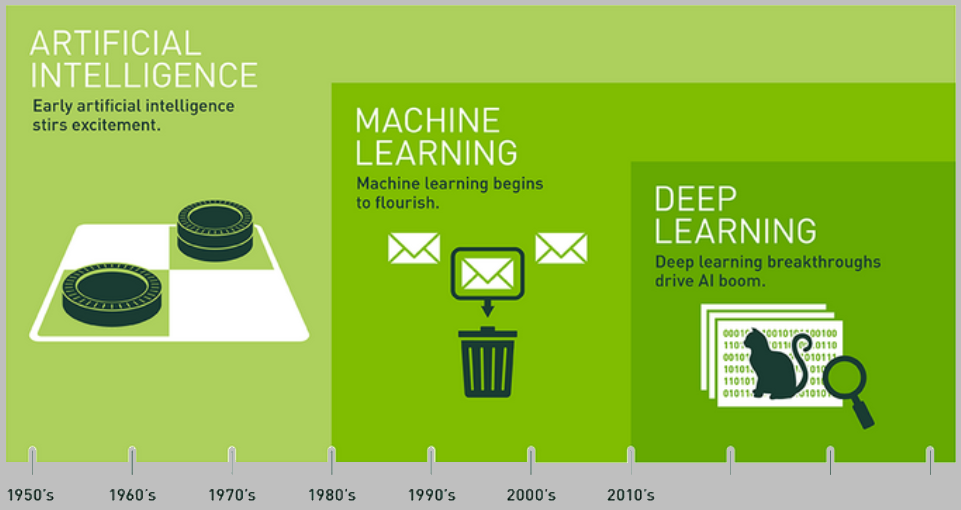
\includegraphics[width=1.1\textwidth]{images/AI-ML-DL_Nvidia-1.png}
  \vspace*{-7mm}
  \center{\tiny (crédit : \href{https://developer.nvidia.com/deep-learning}{developer.nvidia.com/deep-learning})}
\end{frame}
%===============================================================================

\subsection{Intelligence Artificielle}

%===============================================================================
\begin{frame}{Intelligence Artificielle ?}

  \bfdarkchoco{Intelligence Artificielle}
  \footnote{{\tiny utilisé la première fois en 1956 par \href{https://en.wikipedia.org/wiki/John\_McCarthy\_\%28computer\_scientist\%29}{John McCarthy},
      chercheur à Stanford lors de la conférence de Dartmouth}} :
  reste un terme ambigu aux définitions multiples :

  \begin{itemize}

  \item <2-> {\em ''...the science of making computers do things that require intelligence when done by humans.}''
    {\tiny \href{http://www.alanturing.net/turing\_archive/pages/reference\%20articles/what\%20is\%20ai.html}{Alan Turing, 1940}}\\[3mm]    

  \item <2-> {\em ''the field of study that gives computers the ability to learn without being explicitly programmed.''}
        {\tiny  \href{http://infolab.stanford.edu/pub/voy/museum/samuel.html}{Arthur Samuel, 1959}}

  \item <2-> {\em ''A computer program is said to learn from experience E with respect to some class of tasks T and performance measure P,
    if its performance at tasks in T, as measured by P, improves with experience E.''}
    {\tiny \href{https://www.cs.cmu.edu/~tom/}{Tom Mitchell, 1997}}

  \item <2-> Notion d'{\em agent intelligent} ou d'{\em agent rationnel}\\
    {\em ''...agent qui agit de manière à
    atteindre la meilleure solution ou, dans un environnement incertain, la meilleure solution prévisible.}''
    {\tiny  \hyperlink{refRusselNorvig}{Stuart Russel, Peter Norvig, ``Intelligence Artificielle'' 2015}}

  \end{itemize}

\end{frame}
%===============================================================================

%===============================================================================
\begin{frame}{Intelligences Artificielles ?}
  
  \visible<1->{\textbf{\em IA Forte}} ({\em Strong AI})
  \visible<2->{%
    \begin{itemize}
    \item Vise à concevoir des systèmes qui pensent exactement comme les humains.
    \item Peut contribuer à expliquer comment les humains pensent...
    \item On en est encore loin...
    \end{itemize}
    }

  \medskip
  
  \visible<1->{%
    \textbf{\em IA Faible} ({\em Weak AI})}
  \visible<3->{%
    \begin{itemize}
    \item Vise à concevoir des systèmes qui peuvent ``se comporter'' comme des humains.
    \item Ne nous dit rien sur la façon dont les humains pensent.
    \item On y est déjà... On l'utilise tous les jours ! \\
      reconnaissance faciale, vocale, anti-spam, traduction...
    \end{itemize}
    }
   
\end{frame}
%===============================================================================

\section{Machine Learning}

\subsection{Branches}

%===============================================================================
\begin{frame}{{\em Machine Learning} et IA}

  {\small Page extraite de \href{https://medium.com/machine-learning-for-humans/why-machine-learning-matters-6164faf1df12}
  {medium.com/machine-learning-for-humans/...}}\\[2mm]
  
  \hspace*{-10mm}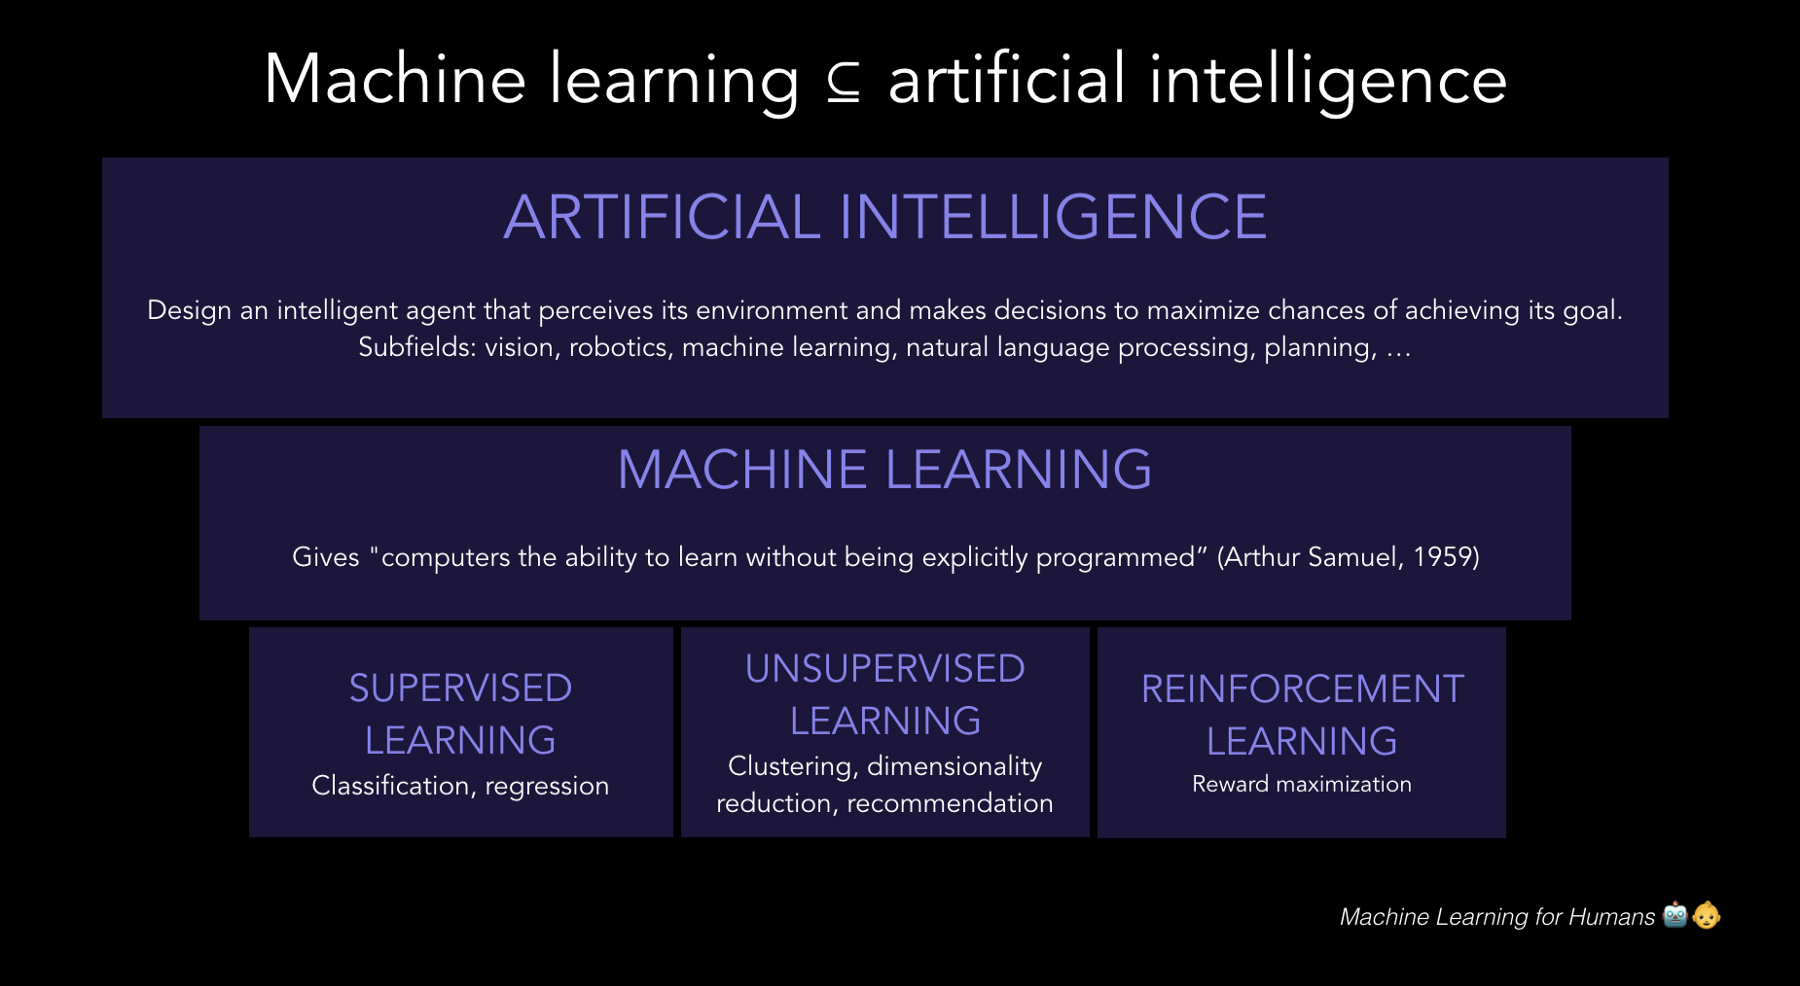
\includegraphics[width=1.2\textwidth]{images/AI-from_MachineLearningForHumans.png}
  \vspace*{-8mm}
  
\end{frame}
%===============================================================================

%===============================================================================
\begin{frame}{Les branches du {\em Machine Learning}}

  \begin{tcolorbox}[title={\em Supervised learning}\\Apprentissage supervisé]
  Requiert des {\bf données labelisées}...
    \begin{itemize}
    \item \textbf{Classification}
      \begin{itemize}
      \item Classification d'images
      \item Détection d'objet sdans des images
      \item Reconnaissance de la parole...
      \end{itemize}
    \item \textbf{Régression}
      \begin{itemize}
      \item Prédiction d'une valeur (continue)...
      \end{itemize}
    \item \textbf{Détection d'Anomalies}
      %% anomaliy detection with supervised laerning suppose that there are no "new annomaly" in the
      %% datat set to process, because the anomalies have been learned and the algorithm will not
      % reconize new anomaly that was not learned...
      \begin{itemize}
      \item Détection de Spam
      \item Manufacturing: reconnaissance de défauts (appris)
      \item Prévision du temps
      \item Classification de maladies...
      \end{itemize}        
    \end{itemize}
  \end{tcolorbox}
\end{frame}
%===============================================================================

%===============================================================================
\begin{frame}{Les branches du {\em Machine Learning}}
  \begin{tcolorbox}[title={\em Unsupervised learning}\\Apprentissage non-supervisé]
    Ne requiert que des données (non labelisées)...
    \begin{itemize}
    \item \textbf{Clustering} -- \textbf{Regroupement} de données non labelisées 
      \begin{itemize}
      \item Data mining, regroupement de données du web, de news...
      \item Regroupement ADN
      \item Traitement de données d'astronomie...
      \end{itemize}        
    \item \textbf{Detection d'Anomalie}
      \begin{itemize}
      \item Détection de fraude
      \item Manufacturing : détection de défauts (même nouveaux)
      \item Monitoring : détéction d'activité anormale (panne, hacker, fraude...)
      \item {\em Fake account} sur Internet...
      \end{itemize}
    \item \textbf{Réduction de dimension}
      \begin{itemize}
      \item Compression de données...
      \end{itemize}
    \end{itemize}
  \end{tcolorbox}    
\end{frame}
%===============================================================================

%===============================================================================
\begin{frame}{Les branches du {\em Machine Learning}}
  \begin{tcolorbox}[title={\em Reinforcement learning}\\Apprentissage par renforcement]
    Un agent (le réseau de neurones) apprend à piloter un environnement (jeu, système mécatronique...)
    \begin{itemize}
    \item \textbf{Contrôle/commande}
      \begin{itemize}
      \item Contrôle de robots, drones...
      \item Financial (stock) trading...
      \end{itemize}        
    \item \textbf{Prise de décision}
      \begin{itemize}
      \item jeux (video games)
      \item analyse financière...
      \end{itemize}
    \end{itemize}
  \end{tcolorbox}    
\end{frame}
%===============================================================================

\subsection{technics}

%===============================================================================
\begin{frame}{Machine Learning et IA}

  %% Excellent: https://www.ibm.com/cloud/learn/machine-learning?lnk=fle
  
  \begin{tcolorbox}[title=Plusieurs approches pour les algorithmes de {\em Machine Learning}]
    {\small
      \begin{minipage}[t]{.55\textwidth}
        Supervised learning:
        \begin{itemize}
        \item Neural Networks
        \item Bayesian inference
        \item Random forest
        \item Decision Tree
        \item Support Vector Machine (SVM)
        \item K-Nearest Neighbor (KNN)
        \item Linear egression
        \item Logistic regression...
        \end{itemize}
      \end{minipage}\begin{minipage}[t]{.5\textwidth}
        Unsupervised learning:
        \begin{itemize}
        \item Neural Networks
        \item Principal Component Analysis (PCA)
        \item Sungular Value Decomposition (SVD)
        \item K-mean clustering
        \end{itemize}
      \end{minipage}
    }
  \end{tcolorbox}    
  
  %  \item Genetic programming
  %    \item Fuzzy logic
  
  \bigskip
  \visible <2->{La suite traite uniquement des \bfdarkchoco{Réseaux de neurones artificiels}.}
\end{frame}
%===============================================================================

\section{NN}

\subsection{Artificial neuron}

%===============================================================================
\begin{frame}{Neurone artificiel}
  
  \tikzset{%
  neuron/.style={
    circle,
    draw,
    minimum size=.7cm,
    font=\normalsize
  },
  squa/.style={
    draw,
    inner sep=2pt,
    font=\normalsize,
    join = by -latex
  },
  }

  
  \begin{tcolorbox}[title=Le modèle informatique du neurone artificiel]  

  \hspace*{-1.cm}\begin{tikzpicture}[x=1.5cm, y=.7cm, >=stealth]

  \node [label=above:\parbox{2cm}{\centering {\em input}\\[2mm]}] at (0, 1.5) (x1)  {$x_1$};
  \node [] at (0, 0.5) (x2) {$x_2$};
  \node [] at (0, -0) (vdots) {$\vdots$};
  \node [] at (0, -0.7) (xn) {$x_n$};
  \node [label=above:\parbox{2cm}{\centering {\em bias}}] at (1.5, 1.8) (bias) {$-1$};
  \node [squa, label=above:{\parbox{2cm}{\centering {\em activation\\function}\\[5mm]}}] at (3.8, 0.15) (F) {$f$};
  \node [label=above:\parbox{2cm}{\centering {\em output}\\[5mm]}] at ((5.5, 0.15) (y) {$y = f(\sum_i{w_{i}\,x_i} - b)$};
  
  \node [neuron/.try] (output) at (1.5,0.15) {{$\displaystyle\Sigma$}};
  
  \draw [o-latex] (x1) -- (output);
  \draw [o-latex] (x2) -- (output);
  \draw [o-latex] (xn) -- (output);
  \draw [o-latex] (bias) -- (output);
  \draw [->] (output) -- (F);
  \draw [->] (F) -- (y);

  \node [] at (1.7,1) () {$b$} ;
  \node [] at (.7,1.1) () {$w_1$} ;
  \node [] at (.7,.5) () {$w_2$} ;
  \node [] at (.7, -0.6) () {$w_n$} ;
  \node [] at (2.6, -.15) () {\small $\sum_i{w_{i}\,x_i} - b$};
\end{tikzpicture}

  \end{tcolorbox}
  
  \visible<2->{Un \bfdarkchoco{neurone artificiel}:
    \begin{itemize}
    \item <2-> reçoit les données d'entrée $(x_{i})_{i=1..n}$ affectées des  \textbf{poids} $(w_i)_{i=1..n}$ ({\em weights}) 
    \item <3-> calcule la \textbf{somme pondérée} de ses entrées moins le biais $\sum_i{w_{i}\,x_i} - b$
    \item <4-> produit en sortie une \textbf{activation} $f(\sum_i{w_{i}\,x_i} - b)$, calculée avec une fonction d'activation $f$ (en général non-linéaire).
    \end{itemize}
  }

\end{frame}
%===============================================================================

\subsection{Activation functions}

%===============================================================================
\begin{frame}{Neurone artificiel}

  La fonction d'activation d'un neurone :
  \begin{itemize}
  \item indroduit un comportement non-linéaire,
  \item fixe la plage de la sortie du neurone,\\
    par exemple $[-1, 1]$, $[0, 1]$ ou encore $[0, \infty[$.
  \end{itemize}    

  \begin{tcolorbox}[title={\small Exemples de fonctions d'activation souvent utilisées}]
    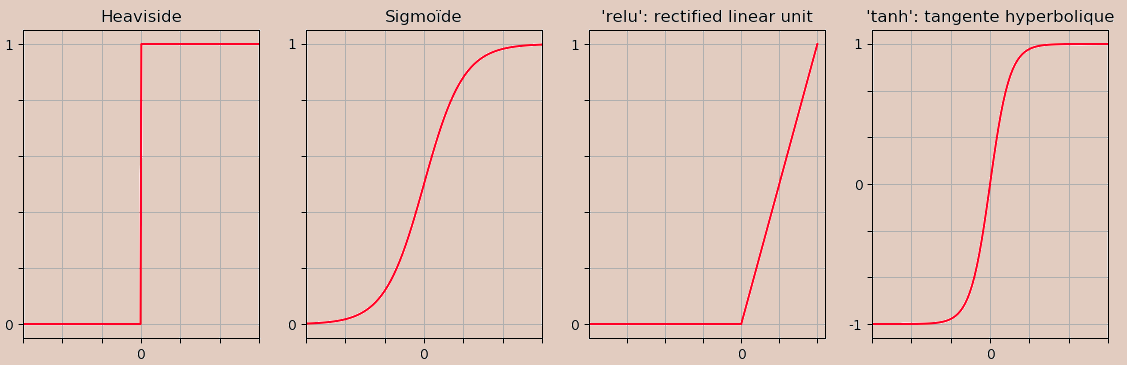
\includegraphics[width=\textwidth]{images/activ_functions-2.png}
  \end{tcolorbox}

  \begin{itemize}
  \item Le biais $b$ fixe le seuil d'activation du neurone.
  \end{itemize}    
   
\end{frame}
%===============================================================================

\subsection{Neural Networks}

%===============================================================================
\begin{frame}{Réseaux de neurones}

  \begin{minipage}{.6\textwidth}
    \begin{itemize}
    \item Les réseaux de neurones sont des assemblages plus ou moins complexes de neurones artificiels organisés en couches.
    \end{itemize}
  \end{minipage}\begin{minipage}{.4\textwidth}
    \vspace*{-6mm}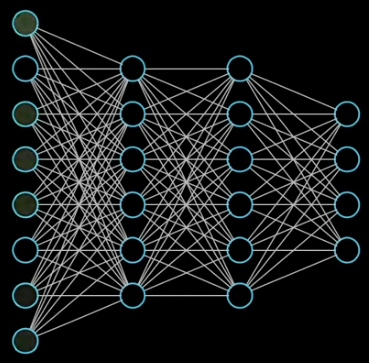
\includegraphics[width=\textwidth]{images/RN.png}
  \end{minipage}
  
  Deux architecture sont très souvent utilisées :
  \begin{itemize}
    \item \textbf{Réseau de Neurones Dense} ({\em Dense Neural Network, RND})\\
      simple, généraliste, peut atteindre des scores de réussite importants.
    \item \textbf{Réseau de Neurones Convolutif} ({\em Convolutional Neural Network, CNN})\\
      plus complexe, spécialisé dans le traitement des images, peut atteindre des scores supérieurs à 99\% dans la reconnaissance d'images.
  \end{itemize}
  
\end{frame}
%===============================================================================

%===============================================================================
\begin{frame}{Données utilisées pour l'APP}

  \begin{itemize}
  \item \href{http://yann.lecun.com/exdb/mnist/}{MNIST} banque de 70000 \textbf{images labellisées}\\
    (60000 images d'entraînement -- 10000 images de test.\\[3mm]
    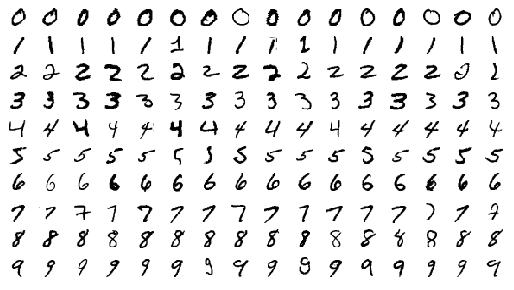
\includegraphics[width=0.6\textwidth]{images/MNIST_digits_sample.png}
  \item Images en ton de gris de 28 $\times$ 28 pixels
  \item Réseau dense $\leadsto$ scores pouvant atteindre 98 \% de succès...
  \item État de l'art pour la reconnaissance d'image : réseau convolutifs
  \end{itemize}       
  
\end{frame}
%===============================================================================

\section{Classification images MNIST par réseau dense}

\subsection{Architecture}

%===============================================================================
\begin{frame}{Réseau de neurones dense}

  {\footnotesize Chaque matrice 28$\,\times\,$28 $\leadsto$ vecteur normalisé de 784 composantes \texttt{float} $\in [0;1]$.}

  \hspace*{-5mm}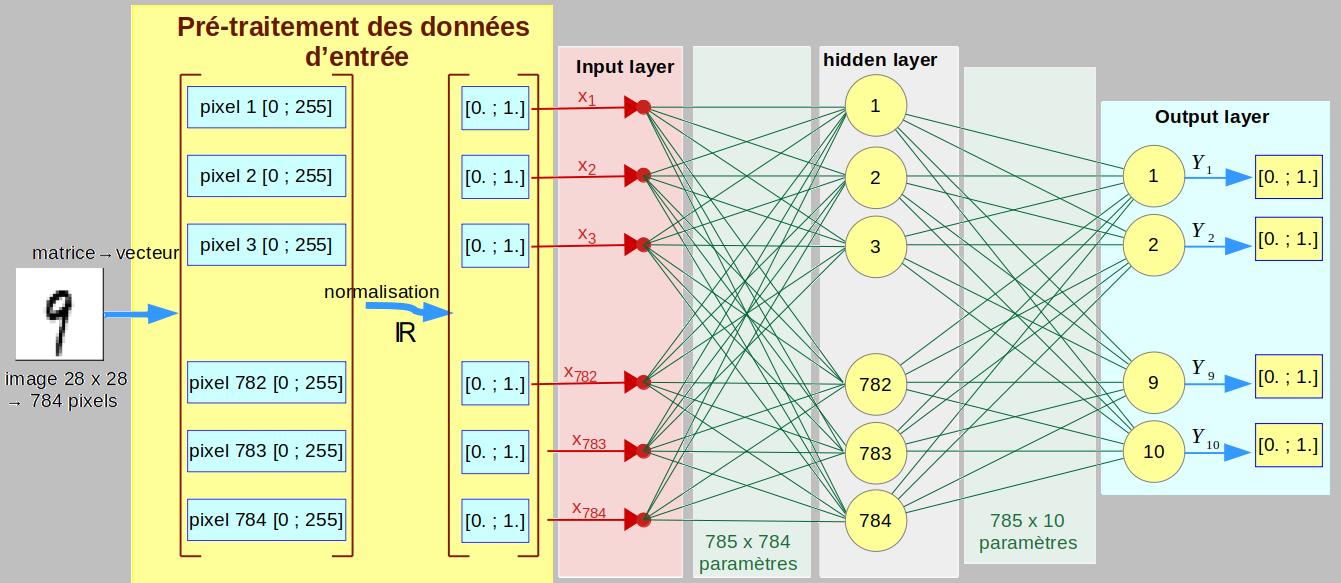
\includegraphics[width=.9\textwidth]{images/archiReseau-2.png}
  
  {\footnotesize
  \begin{itemize}
  \item Couche d'entrée ({\em Input layer}) : fixe la dimension des entrées du réseau, ne comporte aucun neurone.
  \item Couche "cachée" ({\em Hidden layer}) de 784 neurone (on pourrait essayer plus, ou moins...) : reçoit les données d'entrées.
  \item Couche de sortie ({\em Output layer}) : 10 neurones, un pour chaque chiffre à reconnaître.
  \end{itemize}
  }

  
\end{frame}
%===============================================================================

\subsection{Activation functions SoftMax}

%===============================================================================
\begin{frame}{Réseau de neurones dense}
  \vspace*{-2mm}

  \begin{itemize}
    
  \item Dans les couches intermédiaires la fonction d'activation \bfdarkchoco{relu} favorise l'apprentissage du réseau
    \footnote{{\tiny évite le {\em vanishing gradient} qui apparaît dans
        l'algorithme de {\em back propagation}}}.

  \item La classification (dernière couche) utilise la fonction \bfdarkchoco{softmax} :

  \end{itemize}

    
  \begin{tcolorbox}[title=Fonction d'activation {\em softmax}]  

    \begin{minipage}{.45\textwidth}
      \hspace*{-5mm}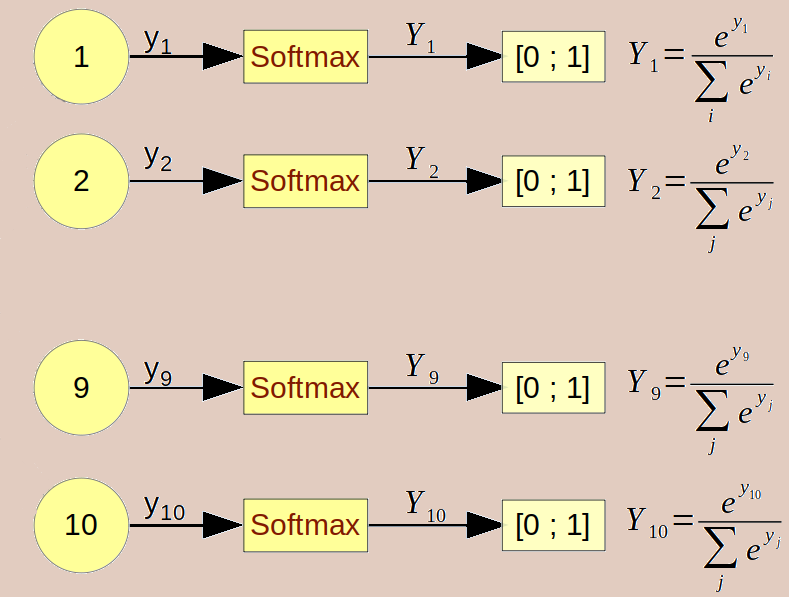
\includegraphics[width=1.\textwidth]{images/softmax-2.png}
    \end{minipage}
    \begin{minipage}{.6\textwidth}
      {\small
        \begin{itemize}
        \item L'activation du neurone $k$ est $Y_k = e^{y_k}/\sum_i{e^{y_i}}$ 
          avec $y_k = \sum_i \omega_i x_i - b$ calculé par le neurone $k$.
        \item Les sorties des neurones s'interprêtent comme des probabilités dans l'intervalle [0,1].
        \end{itemize}
      }
    \end{minipage}
  \end{tcolorbox}

  \vspace*{-1mm}
  \visible<2>{Réponse du réseau $\leadsto$ label associé au neurone de plus grande probabilité.}

\end{frame}
%===============================================================================

\subsection{One-hot coding}

%===============================================================================
\begin{frame}{Réseau de neurones dense}

  \begin{tcolorbox}[title=Codage {\em One-hot} des labels]  

    But : mettre les label des images au format de la sortie du réseau

    {\small
        \begin{itemize}
        \item Labels des images  : \textbf{nombres entiers} de 0 à 9.
        \item Sortie du réseau : \textbf{vecteur de 10 \texttt{float}} dans l'intervalle [0,1] calculés par les fonctions {\em softmax} des 10 neurones de sortie.
        \item Codage {\em one-hot} d'un ensemble ordonné de $N$ labels : \\[1mm]
          - chaque label est représenté par un vecteur à $N$ composantes toutes nulles sauf une égale à $1$,\\
          - le rang du $1$ dans le vecteur associé à un label est le rang du label.
        \end{itemize}
      }
  \end{tcolorbox}  

  \visible<2>{
    \begin{minipage}{.25\textwidth}
      \vspace*{-22mm}\hspace*{-5mm}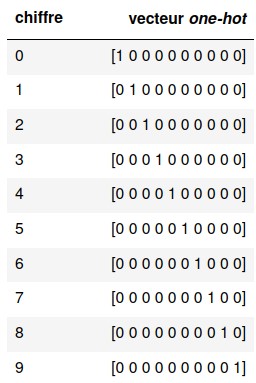
\includegraphics[width=1.1\textwidth]{images/oneHotCoded.png}
    \end{minipage}
    \begin{minipage}{.7\textwidth}
      Le codage {\em one-hot} des labels '0' à '9' donne un vecteur à 10 composantes, comme celui calculé par le réseau de neurones.
    \end{minipage}
  }
    
\end{frame}
%===============================================================================

%===============================================================================
\begin{frame}{1 - Réseau de neurones dense}

  \begin{tcolorbox}[title=Fonction d'erreur : {\em Cross entropy error}]  

    \begin{itemize}
    \item Une image traitée par le réseau $\leadsto$ vecteur $\hat{Y}$ de 10 \texttt{float} à comparer au codage {\em hot-one} $Y$ du label de l'image.
    \item On utilise la fonction d'erreur (ou de perte) {\em cross entropy} adaptée au codage {\em one-hot} : $e(Y,\hat{Y})=-\sum_i Y_i\ log(\hat{Y}_i)$\\
      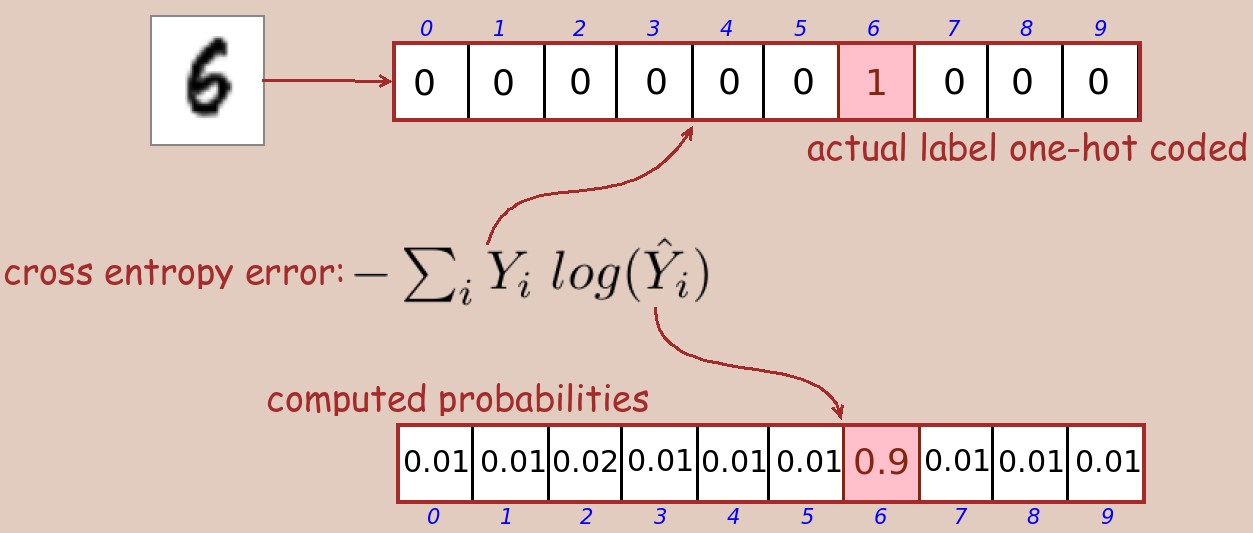
\includegraphics[width=.9\textwidth]{images/CrossEntropyError.png}
    \end{itemize}

  \end{tcolorbox}
  
\end{frame}
%===============================================================================

\subsection{Optimisation}

%===============================================================================
\begin{frame}{1 - Réseau de neurones dense}

  \begin{tcolorbox}[title=Optimisation et {\em Back Propagation}]  

    \begin{itemize}
        \visible<1->{\item Pendant la phase d'apprentissage un algorithme d'optimisation calcule le gradient de la fonction d'erreur 
            par rapport aux poids du réseau.}
        \visible<2->{\item L'algorithme de {\em Back Propagation} \textbf{modifie} les poids du réseau couche par couche grâce au gradient de la fonction d'erreur,
            en itérant de la dernière couche à la première couche. }
        \visible<3->{\item Exemples d'algorithme d'optimisation : 
        \begin{itemize}
        \item Descente de Gradient ({\em Gradient Descent (GD)})
        \item Descente de Gradient Stochastique ({\em Stochastic Gradient Descent (SGD)})
        \item {\em \href{https://arxiv.org/abs/1412.6980}{Adam}} (version améliorée de descente de gradient)...
        \end{itemize}

        {\small Le module \href{https://www.tensorflow.org/api_docs/python/tf/keras/optimizers}{tf.keras.optimizers}
          propose l'implémentation Python de plusieurs algorithmes d'optimisation.}}
      
    \end{itemize}
  \end{tcolorbox}
  
\end{frame}
%===============================================================================

\subsection{Back-propgation algorithm}

%===============================================================================
\begin{frame}{1 - Réseau de neurones dense}

  {\small Visualisation des itérations d'algorithmes de descente de gradient pour une fonction de perte ultra-simple à seulement 2 variables :}\\[2mm]
  \hspace*{25mm}\href{https://github.com/Jaewan-Yun/optimizer-visualization/blob/master/figures/movie9.gif}{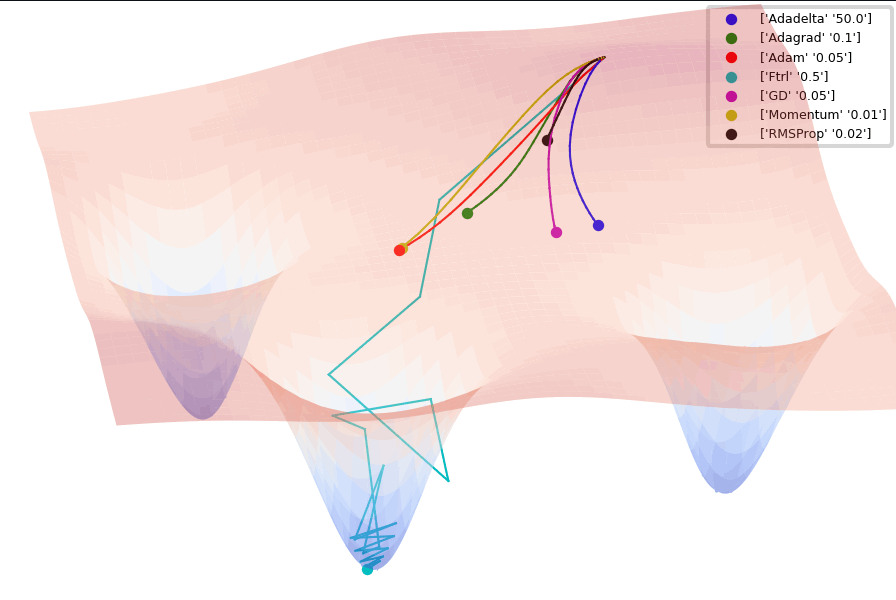
\includegraphics[width=.45\textwidth]{images/adam_plot3D_animated.png}}\\[-2mm]
  %\hspace*{8mm}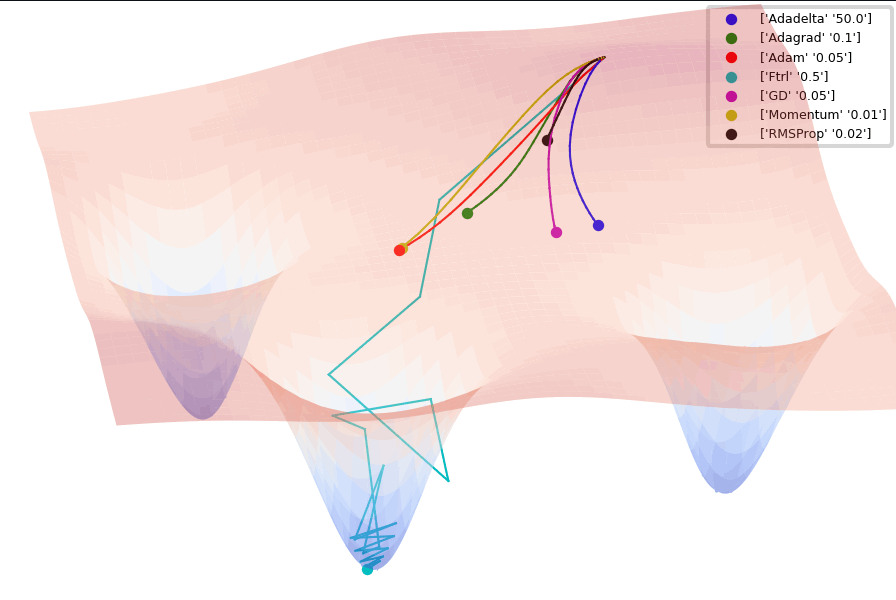
\includegraphics[width=.8\textwidth]{images/adam_plot3D_animated.png}\\[-2mm]
  %\animategraphics[width=.8\textwidth,controls]{10}{./images/Adam-plot3D/movie9/img_}{0}{114}
  \hspace*{25mm}{\tiny (source : \href{https://github.com/Jaewan-Yun/optimizer-visualization}{github.com/Jaewan-Yun/optimizer-visualization})}

  \medskip
  {\small Vidéo d'explication de l'algorithme de {\em back propagation} :}\\
  \hspace*{30mm}\href{https://www.3blue1brown.com/lessons/backpropagation}{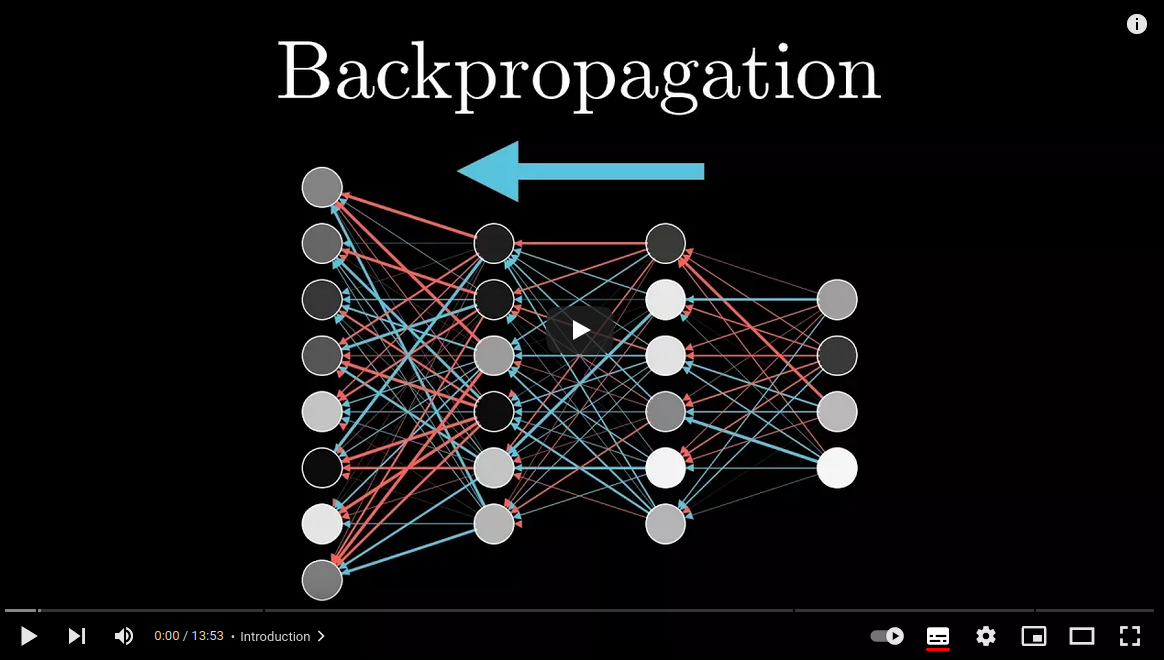
\includegraphics[width=.35\textwidth]{images/video-BackPropagation.png}}
\end{frame}
%===============================================================================

\subsection{Supervised learning}

%===============================================================================
\begin{frame}{}
  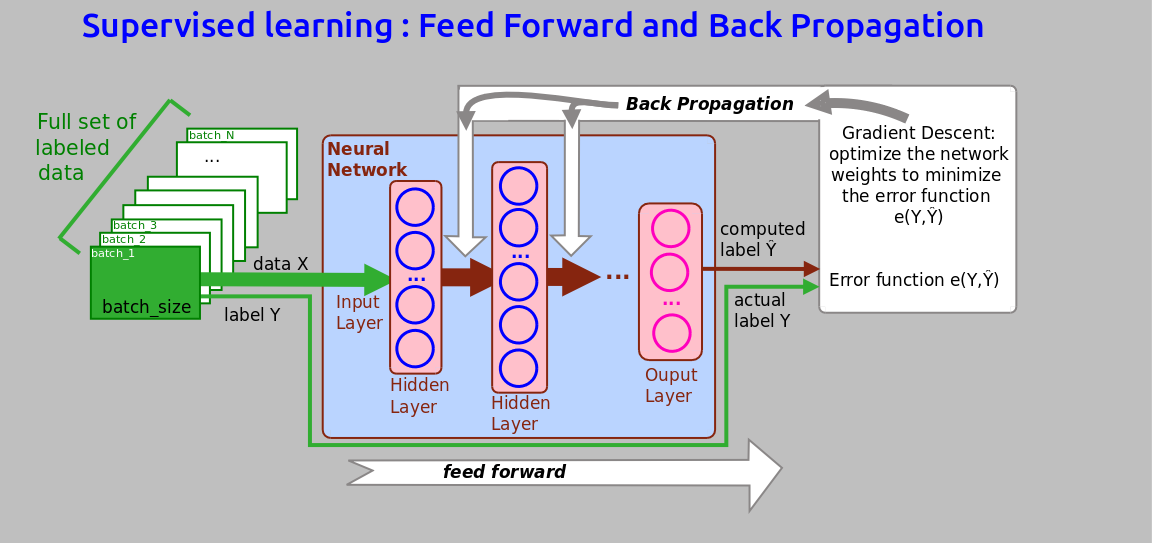
\includegraphics[width=1.2\textwidth]{./images/NetworkTraining.png}
  \begin{itemize}
  \item Le jeu de données est découpé en (mini) {\bf batches} de taille \code{batch\_size}
    \visible<2->{%
    \item Après chaque {\em feed forward} l'algorithme de {\em Back Propagation} modifie les poids
      du réseau de neurone pour minimiser l'erreur $e$.}
  \end{itemize}
\end{frame}
%===============================================================================

\subsection{Supervised learning}

%===============================================================================
\begin{frame}{}
  
  \begin{itemize}
  \item L'entraînement avec le jeu de données complet est répété \code{n\_epoch} fois...
  \end{itemize}
  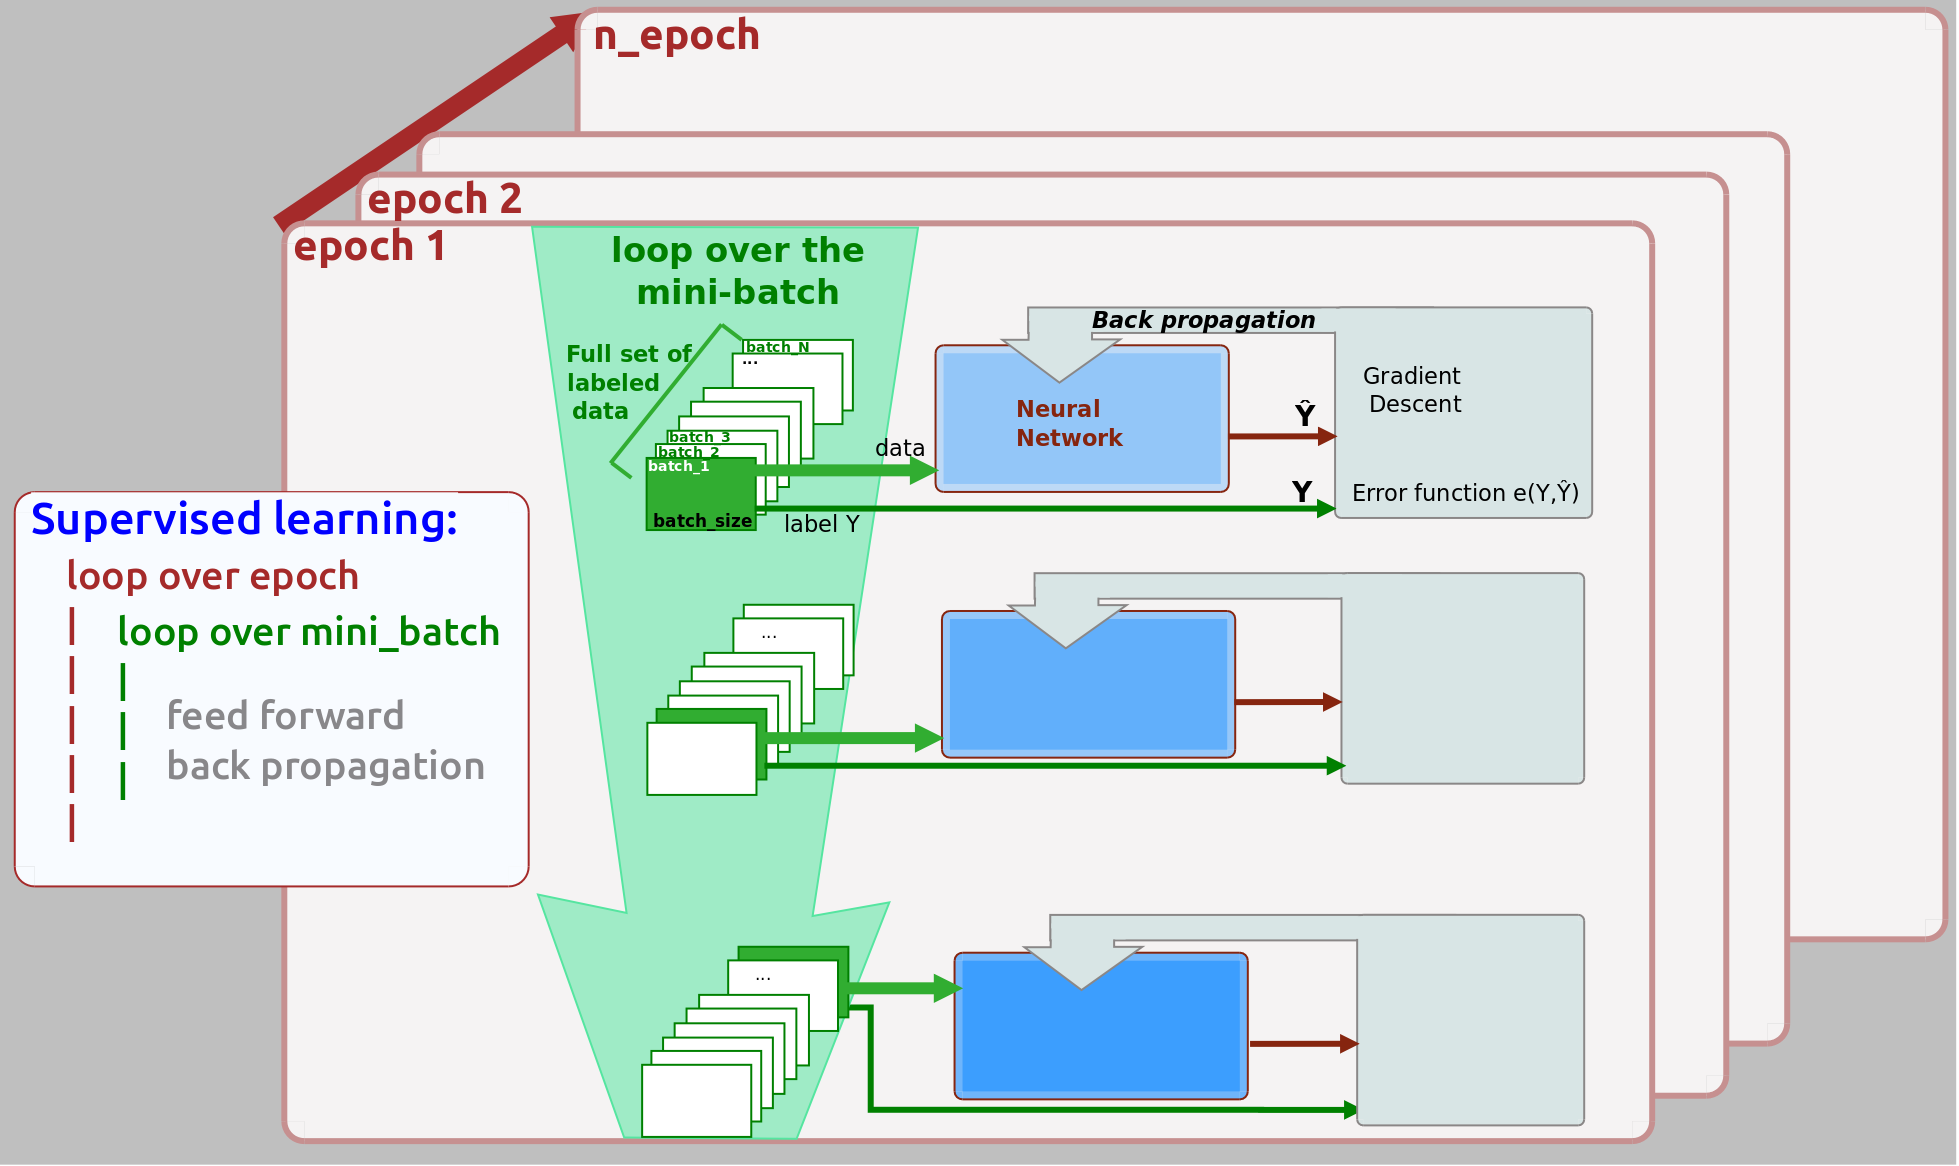
\includegraphics[width=\textwidth]{./images/NetworkTraining_2.png}
  
\end{frame}
%===============================================================================

\section{APP}

%===============================================================================
\begin{frame}{Mise en oeuvre dans l'APP}

  \begin{tcolorbox}[title=1 -- Auto-formation / Réseau dense]
    \begin{itemize}
    \item Les trois {\em notebooks} \DarkBlue{\texttt{ML1\_MNIST.ipynb}}, \DarkBlue{\texttt{ML2\_DNN.ipynb}} et \DarkBlue{\texttt{ML3\_DNN\_suite.ipynb}} visent les savoir-faire :
      \begin{itemize}
      \item charger et pré-traiter les images du MNIST,
      \item construire un réseau de neurones {\bf dense},
      \item entraîner le réseau reconnaître les images du MNIST,
      \item évaluer et exploiter le réseau entraîné.
      \end{itemize}
      
    \item Les modules Python utilisés pour créer les réseaux de neurones et les entraîner sont \href{https://www.tensorflow.org/tutorials}{tensorflow}
      et \href{https://www.tensorflow.org/versions/r2.4/api_docs/python/tf}{keras}.
    \item Les scores obtenus avec des réseaux denses peuvent atteindre 98\% de réussite dans les cas les plus favorables.
    \end{itemize}
  \end{tcolorbox}

\end{frame}
%===============================================================================

%===============================================================================
\begin{frame}{Mise en oeuvre dans l'APP}

  \begin{tcolorbox}[title=2 -- Résolution d'un problème de classification]
    \begin{itemize}
    \item On dispose de données acquises sur un banc de perçage instrumenté.
    \item Une première étape de pré-traitement permet de calculer une quinzaine de
      méta-données ({\em features}) à partir des données brutes acquises avec les capteurs du banc.
    \item L'étude des pré-traitements sera abordée lors de séances de {\em traitement du signal} dédiées.
    \item Le \textbf{problème} proposé : entraîner un réseau de neurones dense à reconnaître le matériau percé
      à partir des méta-données extraites du banc de perçage.
    \end{itemize}
      
  \end{tcolorbox}

\end{frame}
%===============================================================================

\section{Links \& bibliography}

%===============================================================================
\begin{frame}{Vidéographie}

  \hspace*{-3mm}
  \href{https://youtu.be/trWrEWfhTVg}{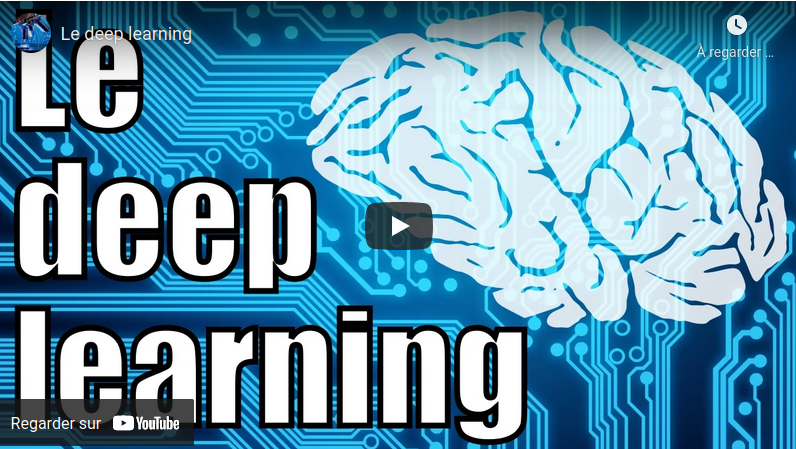
\includegraphics[width=.5\textwidth]{images/video-LeDeepLearning.png}}
  \hfill%
  \href{https://www.3blue1brown.com/lessons/neural-networks}{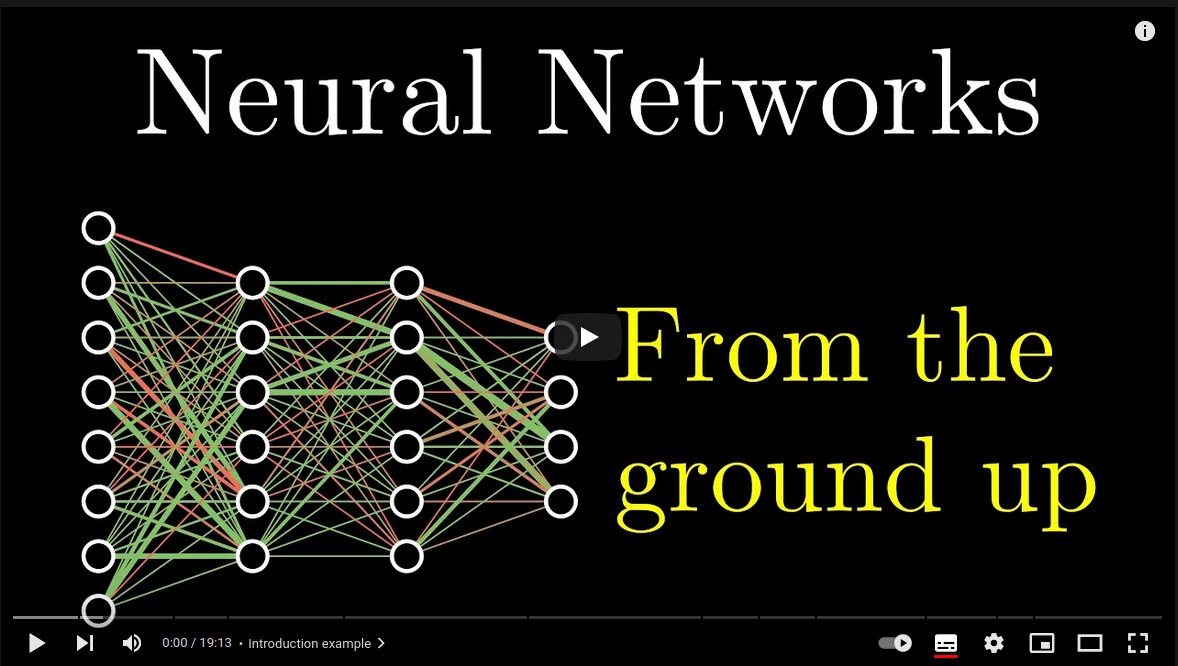
\includegraphics[width=.5\textwidth]{images/video-NeuralNetworks.png}}\\[-2mm]

  {\tiny\hspace*{-2mm}\href{run:./videos/Le deep learning - YouTube.webm}{1/ Local: "Le deep learning - YouTube.webm"}%
    \hfill%
    \href{run:./videos/But what is a neural network.webm}{2/ local : "But what is a neural network.webm"}}\\[2mm]
            
  \hspace*{-3mm}
  \href{https://www.3blue1brown.com/lessons/gradient-descent}{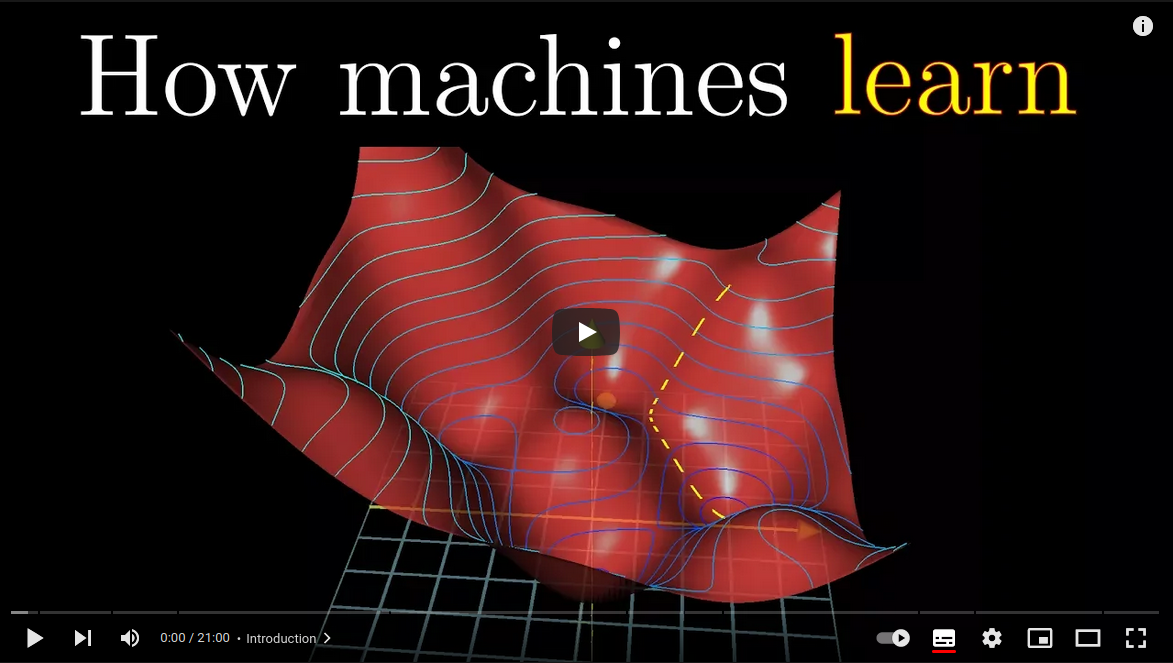
\includegraphics[width=.5\textwidth]{images/video-HowMachineLearn.png}}
  \hfill
  \href{https://www.3blue1brown.com/lessons/backpropagation}{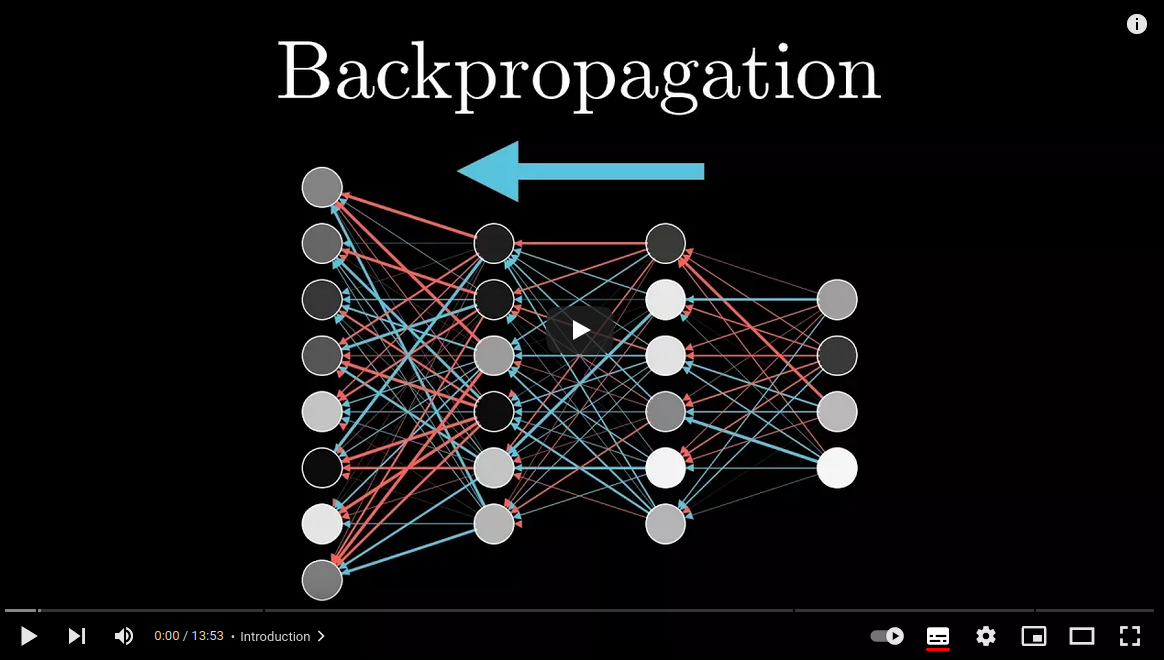
\includegraphics[width=.5\textwidth]{images/video-BackPropagation.png}}\\[-2mm]
  
  {\tiny\hspace*{-3mm}\href{run:./videos/Gradient descent how neural networks learn.webm}{3/ Local: "Gradient descent how neural networks learn.webm"}%
    \hfill%
    \href{run:./videos/What is backpropagation really doing .webm}{4/ Local: "What is backpropagation really doing .webm"}}\\[2mm]
  
\end{frame}
%===============================================================================

%===============================================================================
\begin{frame}{Biliographie}
  
  \noindent\fontsize{8}{8}\selectfont{

    \hspace*{-4mm}\hypertarget{refRusselNorvig}{[1] }%
    {\em Intelligence Artificielle}, 3e édition, PEARSON Education, 2010, ISBN : 2-7440--7455--4,
    \href{http://aima.cs.berkeley.edu/}{aima.cs.berkeley.edu}\\[5mm]


    \hspace*{-4mm}\hypertarget{refStrongWeak-AI}{[2] }%
    {\em What is artificial intelligence (AI), and what is the difference between general AI and narrow AI?}, Kris Hammond, 2015\\
    \href{https://www.computerworld.com/article/2906336/what-is-artificial-intelligence.html}
         {www.computerworld.com/article/2906336/what-is-artificial-intelligence.html}\\[5mm]

    \hspace*{-4mm}\hypertarget{StanfordEncyc}{[3] }%
    {\em Stanford Encyclopedia of Philosophy},
    \href{https://plato.stanford.edu/entries/artificial-intelligence}
         {plato.stanford.edu/entries/artificial-intelligence}\\[5mm]

    \hspace*{-4mm}\hypertarget{DeepLeraning}{[4] }%
    {\em  Deep Learning.}, Goodfellow, Ian; Bengio, Yoshua; Courville, Aaron (2016), MIT Pres, ISBN 9780262035613
  }
  
\end{frame}
%===============================================================================


\end{document}



[ML-01] – JLC  
« Machine Learning for Humans » 
https://medium.com/machine-learning-for-humans

Point d'entrée du site « Machine Learning for Humans », à partir duquel on peut aller sur "A Beginner's Guide to AI/ML" et d'autres documents très intéressants.


[ML-02] – JLC  
« A Beginner’s Guide to AI/ML »
https://medium.com/machine-learning-for-humans/why-machine-learning-matters-6164faf1df12

Cours complet : supervised learning, unsupervised learning, Neural networks & deep learning, reinforcement learning....Version PDF du cours également disponible. sur : https://www.dropbox.com/s/e38nil1dnl7481q/machine_learning.pdf?dl=0

[ML-03] – VG
« ML Basics : Unsupervised, supervised and reinforcement learning »
Article court mais utile pour bien saisir la différence entre supervised, unsupervised et reinforcement learning.
https://medium.com/@machadogj/ml-basics-supervised-unsupervised-and-reinforcement-learning-b18108487c5a

DRL  (Deep Reinforcement Learning)
[DRL-01] – JLC 
« Introduction to Various Reinforcement Learning Algorithms. Part I (Q-Learning, SARSA, DQN, DDPG) »
https://towardsdatascience.com/introduction-to-various-reinforcement-learning-algorithms-i-q-learning-sarsa-dqn-ddpg-72a5e0cb6287

[DRL-02] – VG
https://deepmind.com/blog/deep-reinforcement-learning/
Récapitulatif de ce qu’on sait faire aujourd’hui en DRL fait par DeepMind (un des leaders mondiaux en DRL, concepteurs d’AlphaGo notamment) 

[DRL-03] – JLC
« Demystifying Deeep Reinforcement Learning », Tambet Matiisen
https://neuro.cs.ut.ee/demystifying-deep-reinforcement-learning/
Article très clair et très pédagogique sur ML, RL et DQN.


4 types of deep learning neural networks

There are four types of neural networks:

    Convolutional neural networks: Mostly used for analyzing and classifying images, the architecture of a convolutional neural network is analogous to the organization and connectivity patterns of the visual cortex in the human brain.
    Recurrent neural networks: Used in the field of NLP and sequence prediction problems, the algorithm captures information about previous computations to influence subsequent output.
    Recursive neural networks: These neural networks process input hierarchically in a tree fashion. For example, a recurrent neural network algorithm would analyze a sentence by parsing it into smaller chunks of text or individual words.
    Generative adversarial networks: These networks can generate photographs that appear to be authentic to the human eye by taking photographic data and shaping the elements into realistic-looking objects (e.g., people, animals, locations).


    \subsection{main steps}

%===============================================================================
\begin{frame}{AI recent spots}

  \begin{itemize}
  \item May 11, 1997, the IBM computer \href{https://www-03.ibm.com/ibm/history/ibm100/us/en/icons/deepblue/}{Deep Blue} beat the world chess champion.
  \item 2015 Google trained a conversational agent that could interact with humans, discuss morality, express opinion....
  \item 2015 Google \href{https://deepmind.com}{deepmind} developped an agent that surpassed human performances at 49 Atari games
  \end{itemize}

\end{frame}
%===============================================================================

\footnote{\tiny \hyperlink{DeepLeraning}{[2]} {\em Deep Learning.}, Goodfellow {\em et al.}, Chapitre {\em "6.5 Back-Propagation and Other Differentiation Algorithms"}}
